\documentclass[xcolor=pdflatex,dvipsnames,table]{beamer}
\usepackage{epsfig,graphicx}
\usepackage{palatino}
\usepackage{fancybox}
\usepackage{relsize}
\usepackage[procnames]{listings}
\usepackage{hyperref}
\usepackage{qtree} % needed?
\usepackage{booktabs}
\usepackage{dirtree}
\usepackage[normalem]{ulem}


% fatter TT font
\renewcommand*\ttdefault{txtt}
% another TT, suggested by Alex
% \usepackage{inconsolata}
% \usepackage[T1]{fontenc} % needed as well?


\newcommand{\scale}{0.7}

\newcommand{\todo}[1]{{\emph{TODO: #1}}}
\newcommand{\martin}[1]{{\color{blue} Martin: #1}}
\newcommand{\abcdef}[1]{{\color{red} Author2: #1}}

% uncomment following for final submission
%\renewcommand{\todo}[1]{}
%\renewcommand{\martin}[1]{}
%\renewcommand{\author2}[1]{}

\newcommand{\code}[1]{{\texttt{#1}}}

\hypersetup{
  linkcolor  = black,
%  citecolor  = blue,
  urlcolor   = blue,
  colorlinks = true,
}

\beamertemplatenavigationsymbolsempty
\setbeamertemplate{footline}[frame number]





\newif\ifbook
% shared in slides and book

\lstdefinelanguage{chisel}{
%  morekeywords={abstract,case,catch,class,def,%
%    do,else,extends,false,final,finally,%
%    for,if,implicit,import,match,mixin,%
%    new,null,object,override,package,%
%    private,protected,requires,return,sealed,%
%    super,this,throw,trait,true,try,%
%    type,val,var,while,with,yield},
%  otherkeywords={=>,<-,<\%,<:,>:,\#,@},
  sensitive=true,
  morecomment=[l]{//},
  morecomment=[n]{/*}{*/},
  morestring=[b]",
  morestring=[b]',
  morestring=[b]"""
}

\usepackage{color}
\definecolor{dkgreen}{rgb}{0,0.6,0}
\definecolor{gray}{rgb}{0.5,0.5,0.5}
\definecolor{mauve}{rgb}{0.58,0,0.82}

% Default settings for code listings
%\ifbook
\lstset{%frame=lines,
  language=chisel,
  aboveskip=3mm,
  belowskip=3mm,
  showstringspaces=false,
  columns=fixed, % basewidth=\mybasewidth,
  basicstyle={\small\ttfamily},
  numbers=none,
  numberstyle=\footnotesize,
  % identifierstyle=\color{red},
  breaklines=true,
  breakatwhitespace=true,
  procnamekeys={def, val, var, class, trait, object, extends},
  % procnamestyle=\ttfamily,
  tabsize=2,
  float
}
%\else
%\lstset{%frame=lines,
%  language=chisel,
%  aboveskip=3mm,
%  belowskip=3mm,
%  showstringspaces=false,
%  columns=fixed, % basewidth=\mybasewidth,
%  basicstyle={\small\ttfamily},
%  numbers=none,
%  numberstyle=\footnotesize\color{gray},
%  % identifierstyle=\color{red},
%  keywordstyle=\color{blue},
%  commentstyle=\color{dkgreen},
%  stringstyle=\color{mauve},
%  breaklines=true,
%  breakatwhitespace=true,
%  procnamekeys={def, val, var, class, trait, object, extends},
%  procnamestyle=\ttfamily\color{red},
%  tabsize=2,
%  float
%}
%\fi

\lstnewenvironment{chisel}[1][]
{\lstset{language=chisel,#1}}
{}

\newcommand{\shortlist}[1]{{\lstinputlisting[nolol]{#1}}}

\newcommand{\longlist}[3]{{\lstinputlisting[float, caption={#2}, label={#3}, frame=tb, captionpos=b]{#1}}}

\newcommand{\verylonglist}[3]{{\lstinputlisting[caption={#2}, label={#3}, frame=tb, captionpos=b]{#1}}}


\title{Software-Defined Hardware: Digital Design in the 21st Century with Chisel}
\author{Martin Schoeberl}
\date{\today}
\institute{Technical University of Denmark}

\begin{document}

\begin{frame}
\titlepage
\end{frame}

%\begin{frame}[fragile]{Welcome}
%\begin{itemize}
%\item You can also join this session via the Zoom app
%\item Probably better quality and more functions
%\item The link is in the Whova chat
%%\item \url{https://dtudk.zoom.us/j/61032875012}
%%\item Let us have an introduction round
%\item This shall be interactive: please join with video!
%\item You can ask questions by unmuting and just talking
%\item Use the chat in Zoom to ask questions
%\end{itemize}
%\end{frame}

\begin{frame}[fragile]{Motivating Example:\\
Lipsi: Probably the Smallest Processor in the World}
\begin{itemize}
\item Tiny processor
\item Simple instruction set
\item Shall be small
\begin{itemize}
\item Around 200 logic cells, one FPGA memory block
\end{itemize}
\item Hardware described in Chisel
\item Available at \url{https://github.com/schoeberl/lipsi}
\item Usage
\begin{itemize}
\item Utility processor for small stuff
% \item Could be used for your vending machine
\item In teaching for introduction to computer architecture
\end{itemize}
\item The design took place on the island Lipsi
\end{itemize}
\end{frame}

\begin{frame}[fragile]{The Design of Lipsi on Lipsi}
\begin{figure}
    \centering
    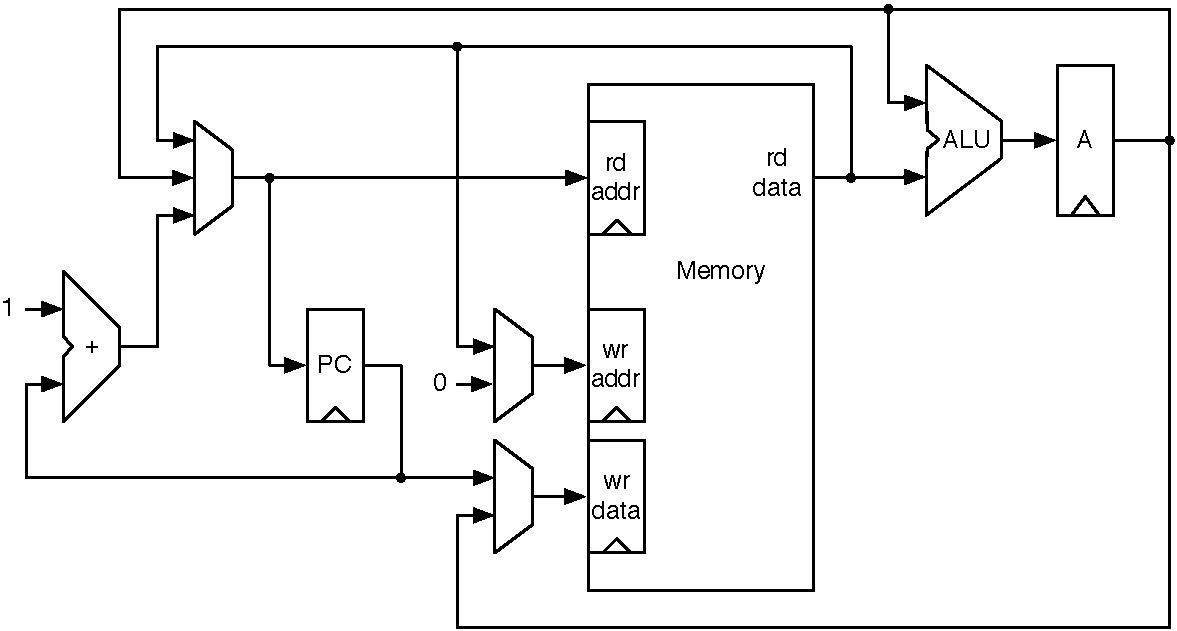
\includegraphics[scale=0.3]{lipsi}
\end{figure}
\end{frame}

\begin{frame}[fragile]{Lipsi Implementation}
\begin{itemize}
\item Hardware described in Chisel
\item Tester in Chisel
\item Assembler in Scala
\begin{itemize}
\item Core case statement about 20 lines
\end{itemize}
\item Reference design of Lipsi as software simulator in Scala
\item Testing:
\begin{itemize}
\item Self testing assembler programs
\item Comparing hardware with a software simulator
\end{itemize}
\item All in a single programming language!
\item All in a single program
\item How much work is this?
\end{itemize}
\end{frame}

\begin{frame}[fragile]{Chisel is Productive}
\begin{itemize}
\item All coded and tested in less than 14 hours!
\end{itemize}
\begin{itemize}
\item The hardware in Chisel
\item Assembler in Scala
\item Some assembler programs (blinking LED)
\item Simulation in Scala
\item Two testers
\end{itemize}
\begin{itemize}
\item BUT, this does not include the design (done on paper)
\end{itemize}
\end{frame}

\begin{frame}[fragile]{Motivating Example: Lipsi, a Tiny Processor}
\begin{itemize}
\item Show in IntelliJ
\end{itemize}
\end{frame}

%\begin{frame}[fragile]{The Slides are Online}
%\begin{itemize}
%\item \url{https://github.com/schoeberl/chisel-book/wiki}
%\end{itemize}
%\begin{figure}
%    \centering
%    \includegraphics[scale=0.5]{slides-link}
%\end{figure}
%\end{frame}

\begin{frame}[fragile]{More on Chisel Success Stories}
\begin{itemize}
\item Before the lockdown at CCC 2020 (in silicon valley)
\item 90 participants
\item More than 30 different (hardware) companies present
\item Several companies are looking into Chisel
\item IBM did an open-source PowerPC
\item \href{https://www.sifive.com/}{SiFive} is a RISC-V startup success
\begin{itemize}
\item High productivity with Chisel
\item Open-source Rocket chip
\end{itemize}
\item Experanto uses the BOOM processor in Chisel
\item Google did a machine learning processor
\item Intel is looking at Chisel
\item Chisel is open-source, if there is a bug you can fix it
\begin{itemize}
\item You can contribute to the Chisel ecosystem
\end{itemize}
\end{itemize}
\end{frame}

\begin{frame}[fragile]{Goals for this Intro}
\begin{itemize}
\item Get an idea what Chisel is
\begin{itemize}
\item Will show you code snippets
\end{itemize}
\item A first high level view of the main features of Chisel
\item Reconsider how to describe hardware
\item Some experience report from usage at DTU
\item Pointers to more information
\item Have your first Chisel design running in an FPGA!
\end{itemize}
\end{frame}

%\begin{frame}[fragile]{Talk abstract}
%
%Date: Tu 19/04/2016, 11:00-12:00
%Room: 123/322
%
%Title: Hardware Design in the 21st Century: with the Object Oriented
%and Functional Language Chisel
%
%Chisel is a hardware construction language implemented as a
%domain specific language in Scala. Therefore, the full power of
%a modern programming language is available to describe hardware
%and, more important, hardware generators. Chisel has been developed
%at UC Berkeley and successfully used for several tape outs of RISC-V.
%Here at DTU we used Chisel in the T-CREST project and in teaching
%advanced computer architecture. Besides presenting small code
%examples in Chisel I will report on experiences on using Chisel in
%the t-CREST project and in teaching.
%
%Martin Schoeberl
%\end{frame}

\begin{frame}[fragile]{Chisel}
\begin{itemize}
\item A hardware \emph{construction} language
\begin{itemize}
\item Constructing Hardware In a Scala Embedded Language
\item If it compiles, it is synthesisable hardware 
\item Say goodby to your unintended latches
\end{itemize}
\item Chisel is not a high-level synthesis language
\item Single source two targets
\begin{itemize}
\item Cycle accurate simulation (testing)
\item Verilog for synthesis
\end{itemize}
\item Embedded in Scala
\begin{itemize}
\item Full power of Scala available
\item But to start with, no Scala knowledge needed
\end{itemize}
\item Developed at UC Berkeley
\end{itemize}
\end{frame}

\begin{frame}[fragile]{The C Language Family}

\Tree[.C [
   [.{\bf Verilog} {\bf SystemVerilog} ]
   [.C++  \emph{SystemC}  ]
   [.Java [.Scala {\bf Chisel} ] ]
   [.C\# ] ] ]
 
\end{frame}

\begin{frame}[fragile]{Other Language Families}

\begin{columns}
\column{0.5\textwidth}
\begin{center}
\Tree[.Algol [.Ada [.{\bf VHDL} ] ] ]
\end{center}
\column{0.5\textwidth}
\begin{center}
\Tree[.Python [.{\bf MyHDL} ] ]
\end{center}
\end{columns}
\end{frame}

\begin{frame}[fragile]{Some Notes on Scala}
\begin{itemize}
\item Object oriented
\item Functional
\item Strongly typed
\begin{itemize}
\item With very good type inference
\end{itemize}
\item Could be seen as Java++
\item Compiled to the JVM
\item Good Java interoperability
\begin{itemize}
\item Many libraries available
\end{itemize}
\end{itemize}
\end{frame}

\begin{frame}[fragile]{Chisel vs. Scala}
\begin{itemize}
\item A Chisel hardware description is a Scala program
\item Chisel is a Scala library
\item When the program is executed it generates hardware
\item Chisel is a so-called \emph{embedded domain-specific language}
\end{itemize}
\end{frame}

\begin{frame}[fragile]{A Small Language}
\begin{itemize}
\item Chisel is a \emph{small} language
\item On purpose
\item Not many constructs to remember
\item The \href{https://github.com/freechipsproject/chisel-cheatsheet/releases/latest/download/chisel_cheatsheet.pdf}{Chisel Cheatsheet} fits on two pages
\item The power comes with Scala for circuit generators
\item With Scala, Chisel can grow with you
\end{itemize}
\end{frame}

\begin{frame}[fragile]{Expressions are Combinational Circuits}
\begin{chisel}
(a | b) & ~(c ^ d)

val addVal = a + b
val orVal = a | b
val boolVal = a >= b
\end{chisel}
\begin{itemize}
\item The usual operations 
\item Simple name assignment with val
\item Width inference
\item Type inference
\item Types: Bits, UInt, SInt, Bool
\end{itemize}
\end{frame}

\begin{frame}[fragile]{Conditional Updates for Combinational Circuits}
\shortlist{../code/comb_elsewhen.txt}
\begin{itemize}
\item Similar to VHDL \code{process} or SystemVerilog \code{always\_comb}
\item Chisel checks for complete assignments in all branches
\item Latches give compile error
\end{itemize}
\end{frame}

\begin{frame}[fragile]{Registers}
\begin{chisel}
val cntReg = RegInit(0.U(32.W))

cntReg := cntReg + 1.U
\end{chisel}
\begin{itemize}
\item Type inferred by initial value (= reset value)
\item No need to specify a clock or reset signal
\end{itemize}
\begin{itemize}
\item Also definition with an input signal connected:
\end{itemize}
\begin{chisel}
val r = RegNext(nextVal) 
\end{chisel}
\end{frame}

\begin{frame}[fragile]{Functional Abstraction}
\begin{chisel}
  def addSub(add: Bool, a: UInt, b: UInt) =
    Mux(add, a+b, a-b)

  val res = addSub(cond, a, b)
  
  def rising(d: Bool) = d && !RegNext(d)
\end{chisel}
\begin{itemize}
\item Functions for repeated pieces of logic
\item May contain state
\item Functions may return \emph{hardware}
\end{itemize}
\end{frame}


\begin{frame}[fragile]{Bundles}
\begin{chisel}
class DecodeExecute extends Bundle {
  val rs1 = UInt(32.W)
  val rs2 = UInt(32.W)
  val immVal = UInt(32.W)
  val aluOp = new AluOp()
}
\end{chisel}
\begin{itemize}
\item Collection of values in named fields 
\item Like struct or record
\end{itemize}
\end{frame}

\begin{frame}[fragile]{Vectors}
\begin{chisel}
val myVec = Vec(3, SInt(10.W))

myVec(0) := -3.S
val y = myVec(2)
\end{chisel}
\begin{itemize}
\item Indexable vector of elements
\item Bundles and Vecs can be arbitrarily nested
\end{itemize}
\end{frame}

\begin{frame}[fragile]{IO Ports}
\begin{chisel}
class Channel extends Bundle {
  val data = Input(UInt(8.W))
  val ready = Output(Bool())
  val valid = Input(Bool())
}
\end{chisel}
\begin{itemize}
\item Ports are Bundles with directions
\item Direction can also be assigned at instantiation:
\end{itemize}
\begin{chisel}
class ExecuteIO extends Bundle {
  val dec = Input(new DecodeExecute())
  val mem = Output(new ExecuteMemory())
}
\end{chisel}
\end{frame}

\begin{frame}[fragile]{Modules}
\begin{chisel}
class Adder extends Module {
  val io = IO(new Bundle {
    val a = Input(UInt(4.W))
    val b = Input(UInt(4.W))
    val result = Output(UInt(4.W))
  })

  val addVal = io.a + io.b
  io.result := addVal
}
\end{chisel}
\begin{itemize}
\item Organization of components
\item IO ports defined as a Bundle named \code{io} and wrapped into an \code{IO()}
\item Created (instantiated) with:
\end{itemize}
\begin{chisel}
val adder = Module(new Adder())
\end{chisel}
\end{frame}

\begin{frame}[fragile]{Hello World in Chisel}
\shortlist{../code/hello.txt}
\end{frame}

\begin{frame}[fragile]{Connections}
\begin{itemize}
\item Simple connections just with assignments, e.g.,
\begin{chisel}
  adder.io.a := ina
  adder.io.b := inb
\end{chisel}
\item Automatic bulk connections between components
\begin{chisel}
  dec.io <> exe.io
  mem.io <> exe.io
\end{chisel}
\end{itemize}
\end{frame}

\begin{frame}[fragile]{Generic Components}
\begin{chisel}
val c = Mux(cond, a, b)
\end{chisel}
\begin{itemize}
\item This is a multiplexer
\item Input can be any type
\end{itemize}
\end{frame}

\begin{frame}[fragile]{Testing}
\begin{chisel}
class CounterTester(c: Counter) extends PeekPokeTester(c) {
  for (i <- 0 until 5) {
    println(i.toString + ": " + peek(c.io.out).toString())
    step(1)
  }
}
\end{chisel}
\begin{itemize}
\item Within Chisel with a tester (= Scala program)
\item May include waveform generation
\item peek and poke to read and set values
\begin{itemize}
\item Remember the BASIC days ;-)
\end{itemize}
\item printf in simulation on rising edge
\begin{chisel}
printf("Counting %x\n", r1)
\end{chisel}
\end{itemize}
\end{frame}

\begin{frame}[fragile]{Component Generation}
\begin{chisel}
val cores = new Array[Module](32)

for (j <- 0 until 32)
  cores(j) = Module(new CPU())
\end{chisel}
\begin{itemize}
\item Use Scala array to collect components
\item Generation with a Scala loop
\end{itemize}
\end{frame}

\begin{frame}[fragile]{Conditional Component Generation}
\begin{chisel}
val icache =
  if (TYPE == METHOD)
    Module(new MCache())
  else if (TYPE == LINE)
    Module(new ICache())
  else
    ChiselError.error("Unsupported Type")
\end{chisel}
\begin{itemize}
\item Use Scala if/else for conditional component types
\item Code example from Patmos
\item We parse an XML file for the configuration
\end{itemize}
\end{frame}

\begin{frame}[fragile]{Logic Generation}
\begin{itemize}
\item Read a file into a table
\begin{itemize}
\item E.g., to read in ROM content for a processor
\end{itemize}
\item Generate a truth table algorithmically
\begin{itemize}
\item E.g., generate binary to BCD translation
\end{itemize}
\item Use the full power of Scala
\end{itemize}
\begin{chisel}
val byteArray = Files.readAllBytes(Paths.get(fileName))
val arr = new Array[Bits](byteArray.length)
for (i <- 0 until byteArray.length) {
  arr(i) = Bits(byteArray(i), 8)
}
val rom = Vec[Bits](arr)
\end{chisel}
\end{frame}

\begin{frame}[fragile]{Tool Flow for Chisel}
\begin{figure}
    \centering
    \includegraphics[scale=0.35]{../figures/flow}
\end{figure}
\end{frame}

\begin{frame}[fragile]{Free Tools for Chisel and FPGA Design}
\begin{itemize}
\item \href{https://adoptopenjdk.net/}{Java OpenJDK 8}
\item \href{https://www.scala-sbt.org/}{sbt, the Scala (and Java) build tool}
\item \href{https://www.jetbrains.com/idea/download/}{IntelliJ (the free Community version)}
\item \href{http://gtkwave.sourceforge.net/}{GTKWave}
\item \href{https://www.xilinx.com/products/design-tools/vivado/vivado-webpack.html}{Vivado WebPACK} or
\item \href{http://www.altera.com/products/software/quartus-ii/web-edition/qts-we-index.html}{Quartus}
\item Nice to have:
\begin{itemize}
\item make, git
\end{itemize}
\item Setup instructions: \url{https://github.com/schoeberl/chisel-lab/blob/master/Setup.md}
\end{itemize}
\end{frame}

\begin{frame}[fragile]{Tool Setup for Different OSs}
\begin{itemize}
\item Windows
\begin{itemize}
\item Use the installers from the websites
\end{itemize}
\item macOS
\begin{itemize}
\item \code{brew install sbt}
\item For the rest, use the installer from the websites
\end{itemize}
\item Linux/Ubuntu
\begin{itemize}
\item \code{sudo apt install openjdk-8-jdk git make gtkwave}
\item Install sbt, see \url{https://github.com/schoeberl/chisel-lab/blob/master/Setup.md}
\item IntelliJ as from the website
\end{itemize}
\end{itemize}
\end{frame}

\begin{frame}[fragile]{Virtual Machine Setup for Chisel}
\begin{itemize}
\item Ubuntu based
\item \href{http://patmos.compute.dtu.dk/patmos-dev.zip}{Ubuntu VM with Quartus} uid: patmos, pwd: patmos
\item \href{https://patmos-download.compute.dtu.dk/de2lab.zip}{Ubuntu VM with Vivado} uid: de2lab, pwd: de2lab
\begin{itemize}
\item But this is VERY large (40 GB for the .zip file)
\end{itemize}
\item Use the  \href{https://www.vmware.com/products/workstation-player.html} {VMWare Workstation Player} (free for Linux and Windows)
\end{itemize}
\end{frame}


\begin{frame}[fragile]{An IDE for Chisel}
\begin{itemize}
\item IntelliJ (Eclipse Scala support is/was shaky)
\item Scala plugin
\item For an Eclipse project: sbt eclipse
\item For IntelliJ: File - New - Project from Existing Sources..., open build.sbt
%\item But you are not compiling with Eclipse\\ and against the Chisel source
\item Show it
\end{itemize}
\end{frame}

\begin{frame}[fragile]{Chisel in the T-CREST Project}
\begin{itemize}
\item Patmos processor rewritten in Chisel
\begin{itemize}
\item As part of learning Chisel
\item 6.4.2013: Chisel: 996 LoC vs VHDL: 3020 LoC
\item But VHDL was very verbose, with records maybe 2000 LoC
\end{itemize}
\item Memory controller, memory arbiters, IO devices in Chisel
\item Several Phd, master, and bachelor projects:
\begin{itemize}
\item Patmos stack cache
\item Method cache for Patmos -- Chisel was relative easy
\item TDM based memory arbiter -- trouble with Chisel
\item RISC stack cache -- no issues with Chisel
\item and more ongoing 
\end{itemize}
\end{itemize}
\end{frame}

\begin{frame}[fragile]{Chisel in Teaching}
\begin{itemize}
\item Using/offering it in Advanced Computer Architecture
\item Spring 2016--2018 all projects have been in Chisel
\item Several Bachelor and Master projects
\item Students pick it up reasonable fast
\item For software engineering students easier than VHDL
\item Switch Digital Electronics 2 at DTU to Chisel (spring semester 2020)
\item Issue of \emph{writing a program} instead of describing hardware remains
\end{itemize}
\end{frame}

\begin{frame}[fragile]{Chisel in Digital Electronic 2}
\begin{itemize}
\item Basic RTL level digital design wit Chisel
\item Chisel testers for debugging
\item Very FPGA centric course
\item Final project is a vending machine
\item All material (slides, book, lab material) in open source
\item Tried to coordinate with introduction to programming (Java)
\begin{itemize}
\item But sometimes I was ahead with Chisel constructs (e.g., classes)
\end{itemize}
\end{itemize}
\end{frame}

\begin{frame}[fragile]{Then there was the Lockdown}
\begin{itemize}
\item Usually one FPGA board per group
\item No group meetings
\item Just virtual labs
\item Can I do something about it with Chisel?
\end{itemize}
\end{frame}

\begin{frame}[fragile]{Teaching Feedback}
\begin{itemize}
\item General positive feedback of the course
\item Most students liked Chisel
\item They also liked the (free) Chisel book
\item Better link to Java programming (same JVM)
\begin{itemize}
\item Similar setup (IDE)
\end{itemize}
\item Lab finish about the same time as last year with VHDL
\begin{itemize}
\item So Chisel is not more productive than VHDL?
\item But we had the Corona lockdown
\end{itemize}
\end{itemize}
\end{frame}

\begin{frame}[fragile]{A Chisel Book}
\begin{figure}
    \centering
    \includegraphics[scale=0.4]{../cover-small}
\end{figure}

\begin{itemize}
\item Available in open access (PDF)
\item In paper from Amazon
\item see \url{http://www.imm.dtu.dk/~masca/chisel-book.html}
\item Source at \url{https://github.com/schoeberl/chisel-book}
\end{itemize}
\end{frame}

\begin{frame}[fragile]{What May Happen with an Open-Source Book}
\begin{figure}
    \centering
    \includegraphics[scale=0.4]{../cover-small-chinese}
\end{figure}

\begin{itemize}
\item A free Chinese translation
\end{itemize}
\end{frame}

\begin{frame}[fragile]{Several Weeks ago I got This}
\begin{figure}
    \centering
    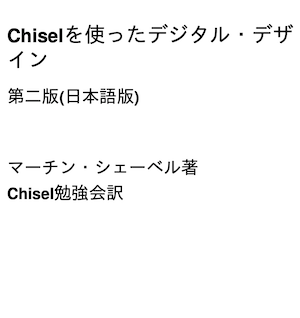
\includegraphics[scale=0.4]{../japanese}
\end{figure}

\begin{itemize}
\item A Japanese translation
\end{itemize}
\end{frame}

\begin{frame}[fragile]{TODO: one more}
\begin{figure}
    \centering
    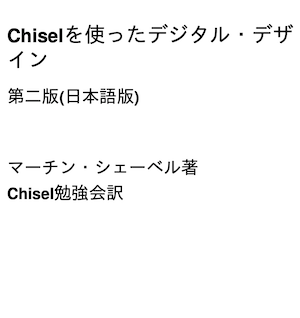
\includegraphics[scale=0.4]{../japanese}
\end{figure}

\begin{itemize}
\item A Japanese translation
\end{itemize}
\end{frame}


\begin{frame}[fragile]{Further Information}
\begin{itemize}
\item \url{https://github.com/schoeberl/chisel-book}
\item \url{https://github.com/schoeberl/chisel-lab}
\item \url{https://www.chisel-lang.org/}
\item \url{https://github.com/ucb-bar/chisel-tutorial}
\item \url{https://github.com/ucb-bar/generator-bootcamp}
%\item Chisel 2 documentation at \url{https://github.com/schoeberl/chisel2-doc}
%\begin{itemize}
%\item Chisel 2.2 Tutorial
%\item Getting Started with Chisel
%\end{itemize}
\item \url{http://groups.google.com/group/chisel-users}
\end{itemize}
\end{frame}


\begin{frame}[fragile]{Hello World in Chisel and Examples}
\begin{chisel}
git clone https://github.com/schoeberl/chisel-examples.git
\end{chisel}
\begin{itemize}
\item or download from \url{https://github.com/schoeberl/chisel-examples}
\item This contains a minimal Chisel project with the blinking LED
\item Has ready to use project files for:
\begin{itemize}
\item Altera DE0
\item Altera DE1
\item Altera DE2-115
\item Altera DE10-Nano
\item BeMicro
\end{itemize}
\item Plus a simple ALU for HW test and showing Chisel Tester
\item Plus some more examples to explore
\end{itemize}
\end{frame}

\begin{frame}[fragile]{What is a Minimal Chisel Project?}
\begin{itemize}
\item Scala class (e.g., \code{Hello.scala})
\item Build info in \code{build.sbt} for \code{sbt}:
\end{itemize}
\begin{chisel}
scalaVersion := "2.11.7"

libraryDependencies += "edu.berkeley.cs" %% "chisel3" % "3.1.2"
\end{chisel}
\begin{itemize}
\item Run the process manually (look into the Makefile)
\end{itemize}
\end{frame}

\begin{frame}[fragile]{Additional Files in the Hello World Example}
\begin{itemize}
\item A \code{Makefile}
\item Optional Verilog or VHDL top level file %\code{verilog/hello\_top.v}
%\begin{itemize}
%\item For reset and possible PLLs
%\item Can also be in VHDL
%\end{itemize}
\item Quartus project files \code{quartus/altde2-115/hello.q\{p|s\}f}
\begin{itemize}
\item List of source files, device and pin assignments
\item plain text files, look into hello.qsf
\end{itemize}
\end{itemize}
\end{frame}

\begin{frame}[fragile]{Summary}
\begin{itemize}
% \item The world is digital
\item Processors do not get much faster -- we need to design domain specific hardware accelerators
\item We need a modern language for hardware/systems design
\item Chisel is a small language
\item Embedding it in Scala gives the power
\item Chisel is good for hardware generators
% \item You can get started with a hardware design in a special course or 4th semester project
\item We can do co-simulation
\end{itemize}
\end{frame}

\begin{frame}[fragile]{Lab Time (Simulation)}
\begin{itemize}
\item Get a blinking LED working in simulation
\item Clone or download the repository from:
\begin{itemize}
\item \url{https://github.com/schoeberl/chisel-lab}
\end{itemize}
\item Follow the instructions from the lab page
\begin{itemize}
\item Start IntelliJ and follow the instructions from the lab page
\item \code{sbt run}
\item Observe the generated Verilog file
\item For simulation change the factor for the counter and run the simulation
\item \code{val CNT\_MAX = (50000 / 2 - 1).U;}
\item \code{sbt test}
\end{itemize}
\item {\bf You have your first Chisel design running in simulation!}
\end{itemize}
\end{frame}

\begin{frame}[fragile]{Lab Time (Basys3)}
\begin{itemize}
\item Get a blinking LED working on the FPGA board
\item Clone or download the repository from:
\begin{itemize}
\item \url{https://github.com/schoeberl/chisel-lab}
\end{itemize}
\item Follow the instructions from the lab page
\begin{itemize}
\item Start IntelliJ and follow the instructions from the lab page
\item \code{sbt run}
\item Create a Vivado project
\item Synthesize with the Play button
\item Configure the FPGA with the Programmer button
\end{itemize}
\item {\bf You have your first Chisel design running in an FPGA!}
\end{itemize}
\end{frame}

\begin{frame}[fragile]{Lab Time (DE2-115)}
\begin{itemize}
\item Get a blinking LED working on the FPGA board
\item Clone or download the repository now
\end{itemize}
\begin{chisel}
git clone \\
   https://github.com/schoeberl/chisel-examples.git
cd chisel-examples/hello-world
make
\end{chisel}
\begin{itemize}
\item Start Quartus
\item Open the project at \code{chisel-examples/hello-world/quartus/altde2-115}
\item Synthesize with the Play button
\item Configure the FPGA with the Programmer button
\item {\bf You have your first Chisel design running in an FPGA!}
\end{itemize}
\end{frame}

\begin{frame}[fragile]{Change the Design}
\begin{itemize}
\item Use \code{gedit}, or the editor you like most
\item Source is in \code{.../src/main/scala/Hello.scala}
\item Change blinking frequency
\item Rerun the example
\item Optional:
\begin{itemize}
\item Change to an asymmetric blinking, e.g., 200 ms on every second 
\item Setup IntelliJ with a Scala project
\end{itemize}
\end{itemize}
\end{frame}


\end{document}

\begin{frame}[fragile]{Title}
\begin{itemize}
\item abc
\end{itemize}
\end{frame}
